\section{Properties of Pure Substances}\label{sec:Properties_Pure_Substances}
Many of the substances that we study in \nameref{def:Thermodynamics} are what we call \nameref{def:Pure_Substance}s.

\begin{definition}[Pure Substance]\label{def:Pure_Substance}
  A \emph{pure substance} is one whose chemical composition is fixed throughout.
  Properties of these substances are completely known, and these properties are completely uniform throughout the substance.
\end{definition}

In general, the pressure of a substance is an exponential function that is dependent on the temperature of the water.
In addition, the pressure of the substance depends on its altitude.
As you increase in altitude, this means that the temperature required to boil the substance at decreases.
All of these are visualized in \Cref{fig:Temp_Pressure_Liquid_Vapor_Curve}.

\begin{figure}[h!tbp]
  \centering
  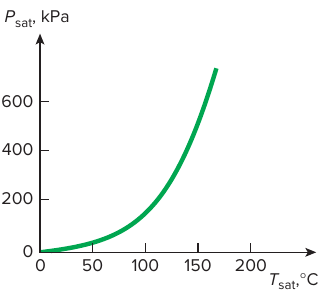
\includegraphics[scale=0.75]{./Temperature_Pressure_Liquid_Vapor_Curve.png}
  \caption{Temperature-Pressure ($\Temp$-$\Pressure$) Liquid-Vapor Curve (\cite[pg. 106]{ThermoTextbook})}
  \label{fig:Temp_Pressure_Liquid_Vapor_Curve}
\end{figure}

\subsection{Phase Changes}\label{subsec:Phase_Changes}
Phase changes in materials are unique, because they maintain a constant temperature \textbf{until} all the material undergoes the phase change, however, the volume increases \textbf{drastically}.

\begin{definition}[Phase Change]\label{def:Phase_Change}
  A \emph{phase change} in a substance is when it changes from one state of matter to another.
  This means a substance goes from solid to liquid, liquid to gas, gas to solid, solid to gas, etc.
  Each of these ``directions'' has a name:
  \begin{description}[noitemsep]
  \item[Solid to Liquid:] Melting/Fusion
  \item[Liquid to Solid:] Solidification/Crystallization
  \item[Liquid to Gas:] Evaporation/Vaporization
  \item[Gas to Liquid:] Condensation
  \item[Solid to Gas:] Sublimation
  \item[Gas to Solid:] Desposition
  \end{description}
\end{definition}

This is visualized as the line between points $A$ and $B$ on the graph in \Cref{fig:Phase_Change}.

\begin{figure}[h!tbp]
  \centering
  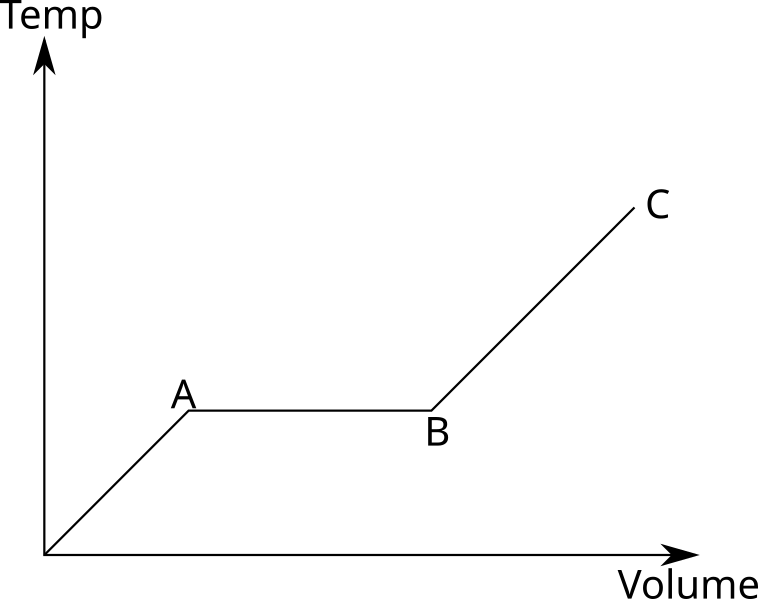
\includegraphics[scale=0.65]{./Phase_Change_Graph.png}
  \caption{Phase Change Graph}
  \label{fig:Phase_Change}
\end{figure}

The line drawn in \Cref{fig:Phase_Change} assumes that the material undergoing the phase change is under \nameref{def:Isobaric} conditions, meaning the pressure is \textbf{not} changing.
However, different pressures (under their own \nameref{def:Isobaric} conditions) will yield different, but similarly shaped, lines as well.

\begin{remark*}
  \Cref{fig:Phase_Change} is also \textbf{NOT} drawn to proportion, as the angle on the first portion of the line is typically \textbf{very} sharp.
  Obviously, \Cref{fig:Phase_Change} is an idealized graph for the temperature-volume graph of a substance and its respective phase change.
  Even though the graph is idealized, it is fine for our needs, and for most needs in \nameref{def:Thermodynamics}.
\end{remark*}

There are several notable points on the graph in \Cref{fig:Phase_Change}:
\begin{enumerate}[noitemsep]
\item Between the origin and point $A$, the substance is called a \nameref{def:Compressed_Liquid}.
  Table A.7 in the textbook has data points for some materials in this state, but the actual values vary very little.
\item At point $A$, the solid begins to boil, becoming a \nameref{def:Saturated_Liquid}, and is denoted $\Fluid{\SpecificVolume}$.
\item Between points $A$ and $B$, the substance is called a \nameref{def:Saturated_Mixture}.
  Here, there are parts of the substance in the liquid phase and the other parts of the substance are in the vapor phase.
  In the textbook, Tables A.4 and A.5 are used here.
\item At point $C$, we have a \nameref{def:Saturated_Vapor} and is denoted $\Vapor{\SpecificVolume}$.
  In the textbook, Tables A.4 and A.5 are used here.
\item Beyond point $C$, the substance is a \nameref{def:Superheated_Vapor}.
  Table A.6 is used in the textbook for substances in this state.
\end{enumerate}

\begin{definition}[Compressed Liquid]\label{def:Compressed_Liquid}
  A \emph{compressed liquid} is a substance, in its liquid state, as it is being heated and gaining volume, until right before it starts to boil.
  Table A.7 in the textbook has data points for some materials in this state, but the actual values vary very little.
  This is because \nameref{def:Pressure} does not change volume much.
  However, temperature \textbf{does} change the volume, therefore, treat compressed liquids as \nameref{def:Saturated_Liquid} at temperature $\Temp$, so use Table A.4.
\end{definition}

\begin{definition}[Saturated Liquid]\label{def:Saturated_Liquid}
  A \emph{saturated liquid} is a substance, starting its \nameref{def:Phase_Change} state between liquid and gas.
  The \nameref{def:Specific_Volume} where a \nameref{def:Compressed_Liquid} begins to boil is denoted $\Fluid{\SpecificVolume}$.
  Tables A.4, and A.5 in the textbook are used here.
\end{definition}

\begin{definition}[Saturated Mixture]\label{def:Saturated_Mixture}
  A \emph{saturated mixture} is a substance in the middle of its \nameref{def:Phase_Change} state betwen a liquid and a gas.
  Parts of the substance in the liquid phase and the other parts of the substance are in the vapor phase.
  In the textbook, Tables A.4 and A.5 are used here.
\end{definition}

\begin{definition}[Saturated Vapor]\label{def:Saturated_Vapor}
  A \emph{saturated vapor} is a substance that has \textbf{JUST} completely undergone its \nameref{def:Phase_Change} to fully become a gas.
  The \nameref{def:Specific_Volume} where this occurs is denoted $\Vapor{\SpecificVolume}$.
  Table A.6 in the textbook contains data points for these vapors.
\end{definition}

\begin{definition}[Superheated Vapor]\label{def:Superheated_Vapor}
  A \emph{superheated vapor} is a substance that has undergone a complete \nameref{def:Phase_Change} to become a gas.
  Here, even if heat is removed, the substance remains a gas until it cools enough or increases in pressure enough to become a \nameref{def:Saturated_Vapor}, then a \nameref{def:Saturated_Mixture} again.
  Table A.6 in the textbook is used to find values for substances in this state.
\end{definition}

\Cref{fig:Phase_Change} can be overlayed with a curve that intersets the different isobars of that \nameref{def:Pure_Substance} based on their \nameref{def:Saturated_Liquid} and \nameref{def:Saturated_Vapor} points.

\begin{figure}[h!tbp]
  \centering
  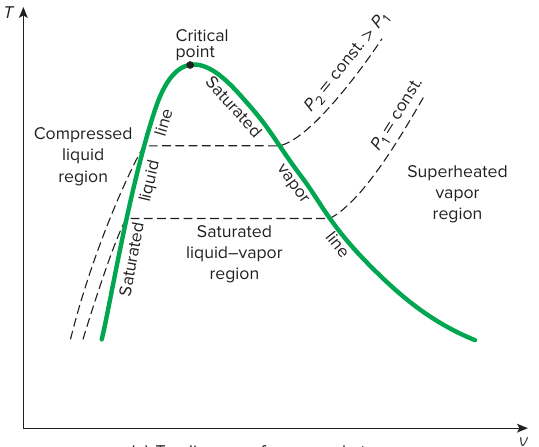
\includegraphics[scale=0.75]{./Temperature_Volume_Diagram.png}
  \caption{Temperature-Volume ($\Temp$-$\Volume$) Diagram (\cite[pg. 110]{ThermoTextbook})}
  \label{fig:Temperature_Pressure_Diagram}
\end{figure}

\begin{figure}[h!tbp]
  \centering
  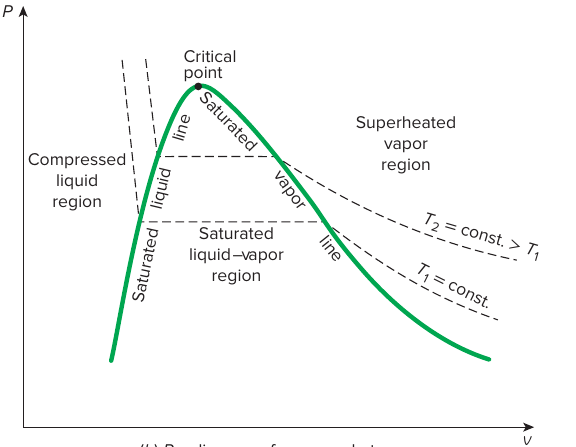
\includegraphics[scale=0.75]{./Pressure_Volume_Diagram.png}
  \caption{Pressure-Volume ($\Pressure$-$\Volume$) Diagram (\cite[pg. 110]{ThermoTextbook})}
  \label{fig:Pressure_Volume_Diagram}
\end{figure}

\begin{definition}[Interpolate]\label{def:Interpolate}
  Many of the values in the tables in the textbook are useful.
  However, sometimes the value we are interested in is \textit{not} in these tables, but between some known entries in the table.
  So, we must \emph{interpolate} a result to use.
  \begin{equation}\label{eq:Interpolate}
    y = y_{0} + (x_{1} - x) \left( \frac{y_{1} - y_{0}}{x_{1} - x_{0}} \right)
  \end{equation}
  \begin{description}[noitemsep]
  \item[$y$] The value we intend to interpolate for.
  \item[$y_{0}$] The ``earlier'' value to use.
    Typically, this is the known data point below our value of interest.
  \item[$y_{1}$] The ``later'' value to use.
    Typically, this is the known data point above our value of interest.
  \item[$x$] The independent value that we are interested in interpolating \textit{at}.
  \item[$x_{0}$] The ``earlier'' value to use.
    Typically, this is the known data point below our value of interest.
  \item[$x_{1}$] The ``later'' value to use.
    Typically, this is the known data point above our value of interest.
  \end{description}
\end{definition}

\begin{example}{Properties of Water}
  Given water at temperature $\Temp = \SI{75}{\degreeCelsius}$ and a pressure $\Pressure = \SI{100}{\kilo\pascal}$.
  What is the water's current state?
  \tcblower{}
  We can start by looking in Table A.4 in the textbook.

  At \SI{75}{\degreeCelsius}, water boils at \SI{38}{\kilo\pascal}.
  This water will \textbf{not} boil at that temperature and pressure.
  Now going to Table A.5, which says that at our pressure, water boils at \SI{99.61}{\degreeCelsius}.

  This means that the water is in its liquid state, and is not in its \nameref{def:Saturated_Mixture} state yet.
\end{example}

\begin{definition}[Enthalpy of Vaporization]\label{def:Enthalpy_Vaporization}
  The \emph{\nameref{def:Specific_Enthalpy} of vaporization} (or \emph{latent heat of vaporization}) represents the amount of \nameref{def:Energy} required to vaporize a unit mass of \nameref{def:Saturated_Liquid} at a given temperature or pressure.
  This value \textbf{decreases} as the temperature and/or pressure increase and becomes $0$ at the critical point.
  This value is denoted using $\SpecificEnthalpy_{fg}$, and is composed using \Cref{eq:Enthalpy_Vaporization} below.
  \begin{equation}\label{eq:Enthalpy_Vaporization}
    \SpecificEnthalpy_{fg} = \SpecificEnthalpy_{f} - \SpecificEnthalpy_{g}
  \end{equation}
\end{definition}

\subsection{Mixtures}\label{subsec:Mixtures}
In the real world, we come across \nameref{def:Mixture}s all the time.
They do not have the same properties as their \nameref{def:Pure_Substance} counterparts.

\begin{definition}[Mixture]\label{def:Mixture}
  A \emph{mixture} is a substance or set of substances that contain at least more than one different \nameref{def:Saturated_Liquid} and \nameref{def:Saturated_Vapor} at a time.
\end{definition}

When a \nameref{def:Saturated_Liquid} is boiling to become a \nameref{def:Saturated_Vapor}, (Points $A$ and $B$ in \Cref{fig:Phase_Change}), all of the liquid \textbf{must} turn to gas first.
This \nameref{def:Process} has a \nameref{def:Quality}.

\begin{definition}[Quality]\label{def:Quality}
  \emph{Quality} is the ratio of a \nameref{def:Mixture} that is a \nameref{def:Saturated_Vapor} to \nameref{def:Saturated_Liquid}.

  \begin{equation}\label{eq:Quality}
    \begin{aligned}
      \text{Quality} &\equiv \frac{\text{Mass of \nameref{def:Saturated_Vapor}}}{\text{Total mass of \nameref{def:Mixture}}} \\
      \Quality &= \frac{\Mass_{Vapor}}{\Mass_{Liquid} + \Mass_{Vapor}}
    \end{aligned}
  \end{equation}

  \Cref{eq:Quality} is always valued $0 \leq \Quality \leq 1$.
  This is like \nameref{subsec:Energy_Efficiency}, $\Efficiency$.
\end{definition}

\begin{definition}[Specific Volume]\label{def:Specific_Volume}
  \emph{Specific volume} is the volume per unit mass of a substance.
  This is typically well-defined for \nameref{def:Saturated_Mixture}s, because the system is in 2 different phases.
  If we are interested in the specific volume of the \nameref{def:Mixture}, we have \Cref{eq:Specific_Volume}.
  \begin{equation}\label{eq:Specific_Volume}
    \SpecificVolume = \frac{\SaturatedVaporVol}{\SaturatedFluidVol}
  \end{equation}

  \begin{description}[noitemsep]
  \item $\SpecificVolume$: The Specific Volume at any point in time during a \nameref{def:Process}.
  \item $\SaturatedVaporVol$: The \nameref{def:Saturated_Liquid} volume.
  \item $\SaturatedFluidVol$: The \nameref{def:Saturated_Vapor} volume.
  \end{description}

  \begin{equation}\label{eq:Specific_Volume_Using_Quality}
    \begin{aligned}
      \Quality &= \frac{\Volume_{Gas}}{\Volume_{Total}} \\
      \SpecificVolume &= (1 - \Quality) \SaturatedFluidVol + \Quality \SaturatedVaporVol \\
      &= \SaturatedFluidVol + \Quality (\SaturatedVaporVol - \SaturatedFluidVol)
    \end{aligned}
  \end{equation}
\end{definition}

From \Cref{eq:Specific_Volume}, it is clear that to get the total volume of \textbf{one phase of the system}, we use \Cref{eq:Single_Phase_Total_Volume}
\begin{equation}\label{eq:Single_Phase_Total_Volume}
  \SpecificVolume \Mass_{Phase} = \Volume_{Phase}
\end{equation}

Now, \Cref{eq:Single_Phase_Total_Volume} only finds the volume for a single phase in the system, but because volume is additive, we can use \Cref{eq:Total_Volume}.
\begin{equation}\label{eq:Total_Volume}
  \SpecificVolume \Mass_{Total} = \Mass_{Liquid} \SaturatedFluidVol + \Mass_{Gas} \SaturatedVaporVol
\end{equation}

In fact, \Cref{eq:Total_Volume} can be re-expressed using \nameref{def:Quality}, which gives us \Cref{eq:Specific_Volume_Using_Quality}.
\begin{align*}
  \SpecificVolume \Mass_{Total} &= \Mass_{Liquid} \SaturatedFluidVol + \Mass_{Gas} \SaturatedVaporVol \\
  \SpecificVolume \Mass_{Total} &= (\Mass_{Total} - \Mass_{Gas}) \SaturatedFluidVol + \Mass_{Gas} \SaturatedVaporVol \\
  \SpecificVolume &= \frac{1}{\Mass_{Total}} \bigl( (\Mass_{Total} - \Mass_{Gas}) \SaturatedFluidVol + \Mass_{Gas} \SaturatedVaporVol \bigr) \\
                                &= \left( 1 - \frac{\Mass_{Gas}}{\Mass_{Total}} \right) \SaturatedFluidVol + \frac{\Mass_{Gas}}{\Mass_{Total}} \SaturatedVaporVol \\
  \Quality &= \frac{\Mass_{Gas}}{\Mass_{Total}} \\
  \SpecificVolume &= (1 - \Quality) \SaturatedFluidVol + \Quality \SaturatedVaporVol \\
  &= \SaturatedFluidVol + \Quality (\SaturatedVaporVol - \SaturatedFluidVol)
\end{align*}

The quantities $\SaturatedFluidVol$ and $\SaturatedVaporVol$ \textbf{are fixed} once pressure and temperature have been established.

\begin{example}{Change in Mixture Properties}
  Suppose there is a pot of water with $\Mass = \SI{3}{\kilo\gram}$ of water at $\Pressure = \SI{101}{\kilo\pascal}$, and temperature $\Temp = \SI{100}{\degreeCelsius}$.
  The pot is sitting at $\Temp$ to start with and continues to heat until all water is evaporated.
  \begin{itemize}[noitemsep]
  \item What is the volume of the water at the start?
  \item What is the \nameref{def:Quality} of the \nameref{def:Mixture} at the start?
  \item If $\Quality=\frac{1}{2}$, what is the volume of the resulting system?
  \item If $\Quality=1$, what is the volume of the resulting system?
  \end{itemize}
  \tcblower{}
  Using the equations we have already, we know
  \begin{equation*}
    \Volume = \SaturatedFluidVol \Mass_{Total}
  \end{equation*}
  From Table A.4 in the textbook, we know $\SaturatedFluidVol = \SI{0.001043}{\meter\cubed\per\kilo\gram}$.
  Thus, we can just plug that value into the equation and solve for $\Volume$.
  \begin{align*}
    \Volume &= \SaturatedFluidVol \Mass_{Total} \\
    \intertext{At this pressure and temperature, the liquid water is not becoming a vapor due to boiling, so $\Mass_{Total} = \Mass_{Liquid}$}
            &= \SI{0.001043}{\meter\cubed\per\kilo\gram} (\SI{3}{\kilo\gram}) \\
            &= \SI{0.003129}{\meter\cubed} \\
            &= \SI{3.129}{\liter}
  \end{align*}

  Now to solve for the ``initial'' \nameref{def:Quality}.
  Because the water has \textbf{\textit{JUST}} reached its \nameref{def:Saturated_Liquid} state, the water has \textbf{begun} boiling, but not yet started to vaporize.
  Thus,
  \begin{equation*}
    \Quality = 0
  \end{equation*}

  We are given the \nameref{def:Quality} of the system, $\Quality=\frac{1}{2}$, meaning we have converted half the \nameref{def:Saturated_Liquid} to vapor.
  We can easily find the mass of the vapor, then find its volume.
  \begin{align*}
    \Quality &= \frac{1}{2} \\
    \intertext{Remember, due to the Law of Conservation of Mass, \textbf{all} \SI{3}{\kilo\gram} of the water remains \textbf{IN} the system!}
      &= \frac{\Mass_{Gas}}{\Mass_{Total}} = \frac{\Mass_{Gas}}{\SI{3}{\kilo\gram}} \\
    \frac{1}{2} &= \frac{\Mass_{Gas}}{\SI{3}{\kilo\gram}} \\
    \Mass_{Gas} &= \SI{1.5}{\kilo\gram} \\
  \end{align*}

  Now that we know the mass of the vaporized liquid, we can use \Cref{eq:Specific_Volume_Using_Quality} to solve for the total volume.
  \begin{align*}
    \SpecificVolume &= \SaturatedFluidVol + \Quality(\SaturatedVaporVol - \SaturatedFluidVol) \\
    \intertext{The value for $\SaturatedFluidVol$ remains constant throughout this entire \nameref{def:Process}, so we can reuse that value. The value for $\SaturatedVaporVol$ is found in Table A.4 from the textbook.}
                    &= \SI{0.001043}{\meter\cubed\per\kilo\gram} + \frac{1}{2} (\SI{1.6720}{\meter\cubed\per\kilo\gram} - \SI{0.001043}{\meter\cubed\per\kilo\gram}) \\
                    &= \SI{0.8365}{\meter\cubed\per\kilo\gram}
  \end{align*}

  Now that we have the \nameref{def:Specific_Volume} of the system, we can find the total volume of the system.
  \begin{align*}
    \Volume_{Total} &= \SpecificVolume \Mass_{Total} \\
                    &= \SI{0.8365}{\meter\cubed\per\kilo\gram} (\SI{3}{\kilo\gram}) \\
                    &= \SI{2509}{\liter}
  \end{align*}

  Remember that $\Volume_{Total}$ contains the volume for \textbf{both} the steam \textbf{and} the water.
  If we are curious about the separate values for each, then we can solve for the individual terms in \Cref{eq:Single_Phase_Total_Volume}.
  \begin{align*}
    \Volume_{Water} &= \Mass_{Water} \SaturatedFluidVol \\
                    &= \SI{1.5}{\kilo\gram} (\SI{0.001043}{\meter\cubed\per\kilo\gram}) \\
                    &= \SI{1.56}{\liter} \\
    \Volume_{Steam} &= \Mass_{Steam} \SaturatedVaporVol \\
                    &= \SI{1.5}{\kilo\gram} (\SI{1.6720}{\meter\cubed\per\kilo\gram}) \\
                    &= \SI{2508}{\liter}
  \end{align*}

  Thus,
  \begin{align*}
    \Volume_{Water} &=  \SI{1.56}{\liter} \\
    \Volume_{Steam} &= \SI{2508}{\liter}
  \end{align*}

  For this last part, $\Quality = 1$, meaning that \textbf{all} the water has become steam.
  Thus, $\Mass_{Water} = \SI{0}{\kilo\gram}$ and $\Mass_{Steam} = \SI{3}{\kilo\gram}$.
  Because we also know $\SaturatedVaporVol = \SI{1.6720}{\meter\cubed\per\kilo\gram}$, we can easily just solve for \Cref{eq:Single_Phase_Total_Volume} as the total volume.
  \begin{align*}
    \Volume_{Total} &= \Volume_{Steam} \\
    \Volume_{Steam} &= \SaturatedVaporVol \Mass_{Steam} \\
                    &= (\SI{1.6720}{\meter\cubed\per\kilo\gram}) (\SI{3}{\kilo\gram}) \\
                    &= \SI{5016}{\liter}
  \end{align*}

  So, after the water has completely become steam, the total volume of the system is $\Volume_{Total} = \SI{5016}{\liter}$.
\end{example}

\begin{example}[Problem 4.23]{What's My State}
  Given certain intensive properties of the \nameref{def:Pure_Substance}, water, fill in the table?
  \begin{enumerate}[noitemsep]
  \item $\Temp = \SI{50}{\degreeCelsius}$ and a volume of $\Volume = \SI{4.16}{\meter\cubed\per\kilo\gram}$.
  \item $\Pressure = \SI{200}{\kilo\pascal}$ and the water is in the \nameref{def:Saturated_Vapor} phase.
  \item $\Temp = \SI{250}{\degreeCelsius}$, $\Pressure = \SI{400}{\kilo\pascal}$, and $\Volume = \SI{0.595}{\meter\cubed\per\kilo\gram}$.
  \item $\Temp = \SI{110}{\degreeCelsius}$, $\Pressure = \SI{600}{\kilo\pascal}$.
  \end{enumerate}
  \tcblower{}
  \begin{center}
    \begin{tabular}{ccccc}
      \toprule
      & Temperature $\si{\degreeCelsius}$ & Pressure $\si{\kilo\pascal}$ & Volume $\si{\meter\cubed\per\kilo\gram}$ & Phase \\
      \midrule
      1 & 50 & 12.352 & 4.16 & \nameref{def:Saturated_Mixture} \\
      2 & 120.21 & 200 & 0.88578 & \nameref{def:Saturated_Vapor} \\
      3 & 250 & 400 & 0.595 & \nameref{def:Superheated_Vapor}/Steam \\
      4 & 110 & 600 & 0.001052 & \nameref{def:Compressed_Liquid} \\
      \bottomrule
    \end{tabular}
  \end{center}

  \begin{enumerate}[noitemsep]
  \item Phase 1:
    \begin{enumerate}[noitemsep]
    \item We need to look at Table A.4 for phase 1's saturated pressure, and find it $\SaturatedPressure$.
    \item Now, looking at the values of $\SaturatedFluidVol$ and $\SaturatedVaporVol$ for water at $\Temp = \SI{50}{\degreeCelsius}$, we see the value we're given is somewhere between those.
      Thus, this is a mixture of a \nameref{def:Saturated_Liquid} and a \nameref{def:Saturated_Vapor}, a \nameref{def:Saturated_Mixture}.
    \end{enumerate}
  \item Phase 2:
    \begin{enumerate}[noitemsep]
    \item We were told a pressure, so we should use Table A.5.
    \item Look in Table A.5 and find $\Pressure = \SI{200}{\kilo\pascal}$, and get the saturation temperature, $\SaturatedTemp$.
    \item They told us it was a \nameref{def:Saturated_Vapor}, so we know the value is somewhere on the saturated vapor line, meaning the volume is the same as $\SaturatedVaporVol$.
    \end{enumerate}
  \item Phase 3:
    \begin{enumerate}[noitemsep]
    \item Because we are given both pressure and temperature, either Table A.4 or Table A.5 is applicable.
    \item However, neither table seems to make much sense, as on the temperature table, the pressure is too low, and on the pressure table, the temperature is too low.
    \item On both tables, our volume is significantly greater than even the $\SaturatedVaporVol$.
    \item Because $\Volume > \SaturatedVaporVol$, we go to Table A.6 for superheated water.
    \item Using Table A.6, we see that $\SaturatedVaporVol$ in the table matches the volume given to us.
    \item This means the water is now in its superheated vapor phase.
    \end{enumerate}
  \item Phase 4:
    \begin{enumerate}[noitemsep]
    \item You can start by using Table A.4 or Table A.5, but I will start with Table A.4.
    \item Find \SI{110}{\degreeCelsius} in the table.
    \item Once there, you'll notice their $\SaturatedPressure$ is \textbf{much} lower than what we were given, so we move to the next table.
    \item So, we move to Table A.5, and the temperature in the table is lower than what we were given, so we move onto the next table.
    \item This means that the temperature is lower than is needed to start boiling the water at \SI{600}{\kilo\pascal} and the pressure is too high for the water to start boiling at \SI{110}{\degreeCelsius}.
    \item This means that it must be a \nameref{def:Compressed_Liquid}.
    \item But, we said to treat \nameref{def:Compressed_Liquid}s as \nameref{def:Saturated_Liquid} at temperature $\Temp$, so use Table A.4 instead.
    \end{enumerate}
  \end{enumerate}
\end{example}

\begin{example}[Problem 4.112]{Changing State of R-134a}
  Given $\Mass = \SI{1}{\kilo\gram}$ of R-134a fills a rigid container of volume $\Volume = \SI{0.1450}{\meter\cubed}$ at an initial temperature of $\Temp_{i} = \SI{-40}{\degreeCelsius}$, at a final pressure of $\Pressure_{f} = \SI{200}{\kilo\pascal}$.
  If the container is heated, determine the inital pressure ($\Pressure_{i}$) and the final temperature ($\Temp_{f}$)?
  \tcblower{}
  \textbf{Concepts:} \\
  The vessel has rigid walls, meaning the vessel's volume will remain constant.
  The \nameref{def:Law_Conservation_Mass} states that the gas's mass will remain constant throughout the \nameref{def:Process}. \\
  \begin{equation*}
    \SpecificVolume = \frac{\Volume}{\Mass}
  \end{equation*}

  Finding a state requires knowing 2 of 3 \nameref{def:Intensive_Property}, ($\Pressure$, $\Temp$, $\SpecificVolume$).

  \textbf{Explore:} \\
  Because both mass and volume are constant, the \nameref{def:Specific_Volume} remains constant.
  Values for R-134a are present in Tables A.11 and A.12 in the textbook, which mirror Tables A.4 and A.5, respectively.

  \textbf{Plan:} \\
  Using $\Pressure$ or $\Temp$ and $\SpecificVolume$, solve for the state.

  \textbf{Solve:} \\
  We use Table A.11 in the textbook, because we are given a temperature.
  So, we know:
  \begin{center}
    \begin{tabular}{cccc}
      \toprule
      $\Temp$ & $\SaturatedPressure$ & $\SaturatedFluidVol$ & $\SaturatedVaporVol$ \\
      \midrule
      \SI{-40}{\degreeCelsius} & \SI{51.25}{\kilo\pascal} & \SI{0.0007053}{\meter\cubed\per\kilo\gram} & \SI{0.36064}{\meter\cubed\per\kilo\gram} \\
      \bottomrule
    \end{tabular}
  \end{center}

  Now, we can also find $\SpecificVolume$:
  \begin{align*}
    \SpecificVolume &= \frac{\Volume}{\Mass} \\
                    &= \frac{\SI{0.1450}{\meter\cubed}}{\SI{1}{\kilo\gram}} \\
                    &= \SI{0.1450}{\meter\cubed\per\kilo\gram}
  \end{align*}

  Now, we notice that $\SpecificVolume$ is somewhere between $\SaturatedFluidVol$ and $\SaturatedVaporVol$, meaning the R-134a is in its \nameref{def:Saturated_Mixture} phase right now.

  We use Table A.12 in the textbook, because we are given a pressure for the final state.
  So, we know:
  \begin{center}
    \begin{tabular}{cccc}
      \toprule
      $\Pressure$ & $\SaturatedTemp$ & $\SaturatedFluidVol$ & $\SaturatedVaporVol$ \\
      \midrule
      \SI{200}{\kilo\pascal} & \SI{-10.09}{\degreeCelsius} & \SI{0.0007381}{\meter\cubed\per\kilo\gram} & \SI{0.099951}{\meter\cubed\per\kilo\gram} \\
      \bottomrule
    \end{tabular}
  \end{center}

  Because we know $\SpecificVolume = \SI{0.1450}{\meter\cubed\per\kilo\gram}$, and we have the values for $\SaturatedFluidVol$ and $\SaturatedVaporVol$, we can tell that the gas is not in a superheated vapor state.
  Because the gas is superheated, we need to use Table A.13 instead.

  That table says that a gas with $\SpecificVolume = \SI{0.14504}{\meter\cubed\per\kilo\gram}$ is at $\SaturatedTemp = \SI{90}{\degreeCelsius}$.

  Thus,
  \begin{align*}
    \Pressure_{i} &= \SI{51.25}{\kilo\pascal} \\
    \Temp_{f} &= \SI{90}{\degreeCelsius}
  \end{align*}
\end{example}

\begin{example}[Problem 4.113]{Changing State of Water English}
  Given $\Mass = \SI{1}{\lbm}$ of water at an initial temperature $\Temp_{i} = \SI{400}{\degreeF}$ fills a weighted piston cylinder device with movable lid of volume $\Volume_{i} = \SI{2.649}{\feet\cubed}$.
  If the vessel is cooled to $\Temp_{f} = \SI{100}{\degreeF}$, determine the final pressure ($\Pressure_{f}$) and the final volume of the container $\Volume_{f}$?
  \tcblower{}
  \textbf{Concepts:} \\
  Weighted piston cylinder devices ensure that the pressure exerted by the fluid remains constant, although we don't know what it is.
  The mass of the water in this problem remained unchanged throughout the \nameref{def:Process} as well.
  We know the initial volume, initial temperature and the final temperature.
  Because we were given each temperature, we know the fluid in the vessel is being cooled.

  \textbf{Explore:} \\
  We want to get 2 of those 3 those \nameref{def:Intensive_Property} ($\Pressure$, $\Temp$, or $\SpecificVolume$).
   We can find the $\SpecificVolume_{i}$ for the initial point in time, because we know the volume of the vessel initially and the mass is constant.
  We also know the initial temperature, so we have all the \nameref{def:Intensive_Property}s that we need to solve for the initial state.

  \textbf{Plan:} \\
  Use Table A.4E to find $\Pressure$.
  Because the pressure is constant, we can use $\Pressure$ and the final temperature $\Temp_{f}$ to solve for the final state's $\Volume_{f}$.

  \textbf{Solve:} \\
  Fome Table A.4E, we can find and know
  \begin{center}
    \begin{tabular}{cccc}
      \toprule
      $\Temp$ & $\SaturatedPressure$ & $\SaturatedFluidVol$ & $\SaturatedVaporVol$ \\
      \midrule
      \SI{400}{\degreeF} & \SI{247}{\psia} & \SI{0.01864}{\feet\cubed\per\lbm} & \SI{1.864}{\feet\cubed\per\lbm} \\
      \bottomrule
    \end{tabular}
  \end{center}

  We also know that the \nameref{def:Specific_Volume} of the water is:
  \begin{align*}
    \SpecificVolume &= \frac{\Volume}{\Mass} \\
                    &= \frac{\SI{2.649}{\feet\cubed}}{\SI{1}{\lbm}} \\
                    &= \SI{2.649}{\feet\cubed\per\lbm} \\
  \end{align*}

  Because $\SpecificVolume > \SaturatedVaporVol$, we know that the fluid is a superheated vapor, steam.

  Now, because the fluid is a superheated vapor, we need to use Table A.6E to find the pressure that the water/steam is under.
  Using the temperature and the \nameref{def:Specific_Volume} of the water, we look those values up in Table A.6E, we see that $\Pressure = \SI{180}{\psia}$.
  The saturation pressure $\SaturatedTemp = \SI{373}{\degreeF}$, which means that the final temperature $\Temp_{f}$ is likely a liquid.

  Because the water is likely a liquid at its final temperature, we use Table A.4E and look up the value of water at \SI{100}{\degreeF}.
  \begin{center}
    \begin{tabular}{cccc}
      \toprule
      $\Temp$ & $\SaturatedPressure$ & $\SaturatedFluidVol$ & $\SaturatedVaporVol$ \\
      \midrule
      \SI{100}{\degreeF} & \SI{0.95052}{\psia} & \SI{0.01613}{\feet\cubed\per\lbm} & \SI{349.83}{\feet\cubed\per\lbm} \\
      \bottomrule
    \end{tabular}
  \end{center}

  If we use the pressure we got from Table A.6E $\Pressure = \SI{180}{\psia}$, and look that value up in Table A.5E, we see that $\SaturatedTemp = \SI{373.07}{\degreeF}$ to even boil the water.
  This likely means that the water is a \nameref{def:Compressed_Liquid}, and because of our rule, $\SpecificVolume_{f} = \SI{0.01613}{\feet\cubed\per\lbm}$.
  Therefore, by multiplying $\SpecificVolume_{f}$ by the mass of the water, we can find the volume it is consuming.
  \begin{align*}
    \Volume_{f} &= \SpecificVolume_{f} m \\
                &= \SI{0.01613}{\feet\cubed\per\lbm} (\SI{1}{\lbm}) \\
                &= \SI{0.01613}{\feet\cubed}
  \end{align*}
\end{example}

%%% Local Variables:
%%% mode: latex
%%% TeX-master: "../../MMAE_320-Thermo-Reference_Sheet"
%%% End:


\subsection{Ideal Gas Equation}\label{subsec:Ideal_Gas_Equation}
The Ideal Gas Equation is used when:
\begin{itemize}[noitemsep]
\item We have dry air.
\item Air is \textbf{not} good under high pressures, like in turbines.
\item Not good on for liquid water.
\item Can occasionally be used for steam, when the pressure is $\Pressure \leq \SI{10}{\kilo\pascal}$.
\item Not good for steam at high temperatures or pressures.
\item Good for the noble gases, and hydrogen.
\end{itemize}

\begin{equation}\label{eq:Ideal_Gas_Equation}
  \Pressure \SpecificVolume = \GasConstant \Temp
\end{equation}
where
\begin{description}[noitemsep]
\item $\Pressure$: The \textbf{absolute} pressure.
\item $\SpecificVolume$: The \nameref{def:Specific_Volume}.
\item $\GasConstant$: Gas constant, specified in terms of gases and units.
\item $\Temp$: \textbf{Absolute} temperature (\si{\kelvin} or \si{\rankine}).
\end{description}

There is an alternative to \Cref{eq:Ideal_Gas_Equation}, \Cref{eq:Ideal_Gas_Equation-Mass}.
\begin{equation}\label{eq:Ideal_Gas_Equation-Mass}
  \Pressure \Volume = \Mass \GasConstant \Temp
\end{equation}

\begin{example}[Problem 4.79]{Ideal Gas in Tire}
  The air in a tire has its temperature and pressure measured, as the pressure inside the tire depends on the temperature of the air in the tire.
  Initially, at $\Temp_{i} = \SI{25}{\degreeCelsius}$ the pressure is $\Pressure_{i, \text{Gage}} = \SI{210}{\kilo\pascal}$.
  The volume of the tire is $\Volume = \SI{0.025}{\meter\cubed}$.
  Determine the air pressure in the tire when the tmeperature is $\Temp_{f} = \SI{50}{\degreeCelsius}$?
  Also determine the amount of air that must be let out to restore the original pressure at the new temperature, assuming $\Pressure_{atm} = \SI{100}{\kilo\pascal}$?
  \tcblower{}
  \textbf{Concepts:} \\
  \begin{itemize}[noitemsep]
  \item The tire warms up when driven.
    \begin{equation*}
      \Temp_{i} = \SI{25}{\degreeCelsius} \to \Temp_{f} = \SI{50}{\degreeCelsius}
    \end{equation*}
  \item Air is an ideal gas.
  \item The pressure of the outside air is $\Pressure_{atm} = \SI{100}{\kilo\pascal}$
  \item We are given an initial volume, but no final volume.
  \item We are given a gage pressure, which is the atmospheric pressure plus the pressure in the tire.
    \begin{equation*}
      \Pressure_{\text{gage}} = \Pressure_{abs} - \Pressure_{atm}
    \end{equation*}
  \end{itemize}

  \textbf{Explore:} \\
  The \nameref{subsec:Ideal_Gas_Equation} needs both $\Pressure_{abs}$ and $\Temp_{abs}$.
  We should use \Cref{eq:Ideal_Gas_Equation-Mass}, because we need to know how much air to let out.
  \begin{equation*}
    \Pressure \Volume = \Mass \GasConstant \Temp
  \end{equation*}
  The volume is either unchanged, or changes very little.
  \begin{equation*}
    {\left( \frac{\Pressure \Volume}{\Temp} \right)}_{i} = {\left( \frac{\Pressure \Volume}{\Temp} \right)}_{f}
  \end{equation*}
\end{example}

%%% Local Variables:
%%% mode: latex
%%% TeX-master: "../../MMAE_320-Thermo-Reference_Sheet"
%%% End:


%%% Local Variables:
%%% mode: latex
%%% TeX-master: "../MMAE_320-Thermo-Reference_Sheet"
%%% End:
